\section{Tecnologías}
Para el desarrollo del proyecto se propone utilizar las siguientes tecnologías que permitirán lograr los objetivos propuestos en el sistema. Las ventajas que representan para el desarrollo son descritas a continuación.

	\begin{table}[h]
	\begin{center}
	  \begin{tabular}{ | c | p{10cm} | }
	 	% Neo4j, Java(OGM, JSP, Spring), Bootstrap, JQuery, Git
	    \toprule
	    Nombre & Ventajas \\
	    \midrule
	    \raisebox{-\totalheight}{
\includegraphics[width=0.3\textwidth, height=25mm]{images/java}} &
	    \begin{itemize}[topsep=0pt]
	      \item  
	      \item JSP: 
	      \item Spring
	      \item Object Graph Mapping (OGM):
	    \end{itemize} \\
	    \midrule
	    \raisebox{-\totalheight}{
\includegraphics[width=0.3\textwidth, height=30mm]{images/neo4j}} &
	    \begin{itemize}[topsep=0pt]
	      \item  
	    \end{itemize} \\
	    \midrule    
	    \raisebox{-\totalheight}{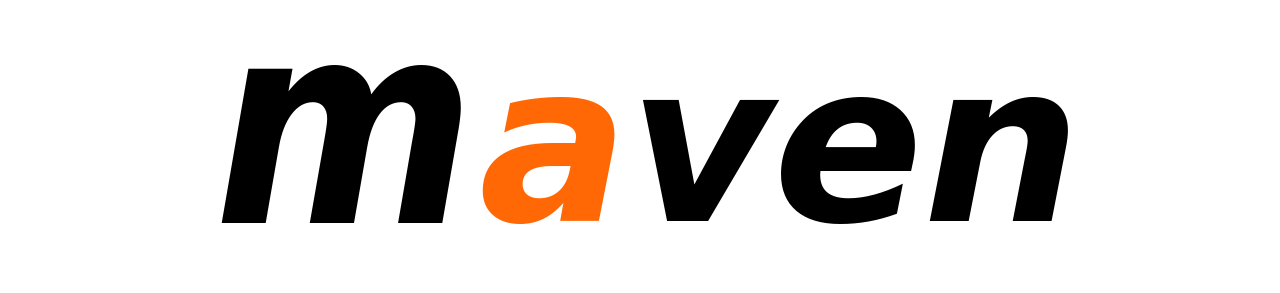
\includegraphics[width=0.3\textwidth, height=15mm]{images/maven}} &
	    \begin{itemize}[topsep=0pt]
	      \item 
	    \end{itemize} \\
	    \midrule
	    \raisebox{-\totalheight}{
\includegraphics[width=0.3\textwidth,height=1.6cm]{images/jquery}} &
	    \begin{itemize}[topsep=0pt]
	      \item  
	    \end{itemize} \\
	    \midrule
	    \raisebox{-\totalheight}{
\includegraphics[width=0.3\textwidth,height=1.6cm]{images/git}} &
	    \begin{itemize}[topsep=0pt]
	      \item  
	    \end{itemize} \\
	    \bottomrule
		\end{tabular}
  	\caption{Descripción de las tecnologías}
  	\label{Descripción de las tecnologías}
  	\end{center}
	\end{table}
